\chapter{Clasificar los seres vivos}\label{ch:g3:sorting-living-things}

Vuelca una caja de botones variados sobre la mesa y tus manos empiezan
a clasificarlos solas: los grandes con los grandes, los rojos con los
rojos, los de cuatro agujeros con los de cuatro agujeros. Los
naturalistas sintieron ese mismo impulso ante el revoltijo de
escarabajos, pájaros, helechos y \omterm{prop:g3:sorting-living-things:groups}{peces} del mundo vivo --- y clasificar
con cuidado a los \omterm{def:g1:living-or-not:living}{seres vivos} resultó ser una de las ideas más
poderosas de la \omterm{def:g1:living-or-not:living}{biología}.

\section{Para clasificar hace falta una regla}

\begin{definition}[Clasificar y criterios]\label{def:g3:sorting-living-things:criterion}
\emph{Clasificar}\index{clasificación} una colección es juntar las
cosas que van juntas. Un \emph{criterio}\index{criterio} es la regla
que se usa para clasificar --- ``tiene seis patas'', ``tiene \omterm{def:g1:animals-around-us:covering}{plumas}''.
Un buen criterio para los \omterm{def:g1:living-or-not:living}{seres vivos} es un rasgo del cuerpo que se
puede \emph{observar}: algo que el \omterm{def:g1:animals-around-us:animal}{animal} o la \omterm{def:g1:plants-around-us:plant}{planta} \emph{tiene}, y
no el sitio donde vive ni lo que esté haciendo en ese momento.
\end{definition}

\begin{example}[Dos clasificaciones de los mismos animales]\label{ex:g3:sorting-living-things:two}
Coge el gato, el pato, la trucha y la mariquita. Clasificados por
``vive cerca del agua'': el pato y la trucha juntos. Clasificados por
``tiene \omterm{def:g1:animals-around-us:covering}{plumas}'': el pato se queda solo. Las dos son clasificaciones
--- pero solo la segunda usa el cuerpo del propio \omterm{def:g1:animals-around-us:animal}{animal}, y esa es la
clase en la que confían los biólogos: un \omterm{def:g1:animals-around-us:animal}{animal} se puede mudar de
casa, pero no puede cambiar sus \omterm{def:g1:animals-around-us:covering}{plumas} por escamas.
\end{example}

\begin{remark}[¿Por qué no clasificar por la casa o por el menú?]\label{rem:g3:sorting-living-things:why}
El \omterm{def:g2:where-animals-live:habitat}{hábitat} y el menú cambian con las estaciones y con la suerte --- el
mirlo del \cref{ch:g2:what-animals-eat} pasa de las lombrices a las
bayas sin convertirse en otro \omterm{def:g1:animals-around-us:animal}{animal}. Los rasgos del cuerpo se quedan.
Por eso ``lo que tiene'' gana a ``lo que hace'' como regla de
\omterm{def:g3:sorting-living-things:criterion}{clasificación}.
\end{remark}

\section{Los grandes grupos de animales}

\begin{proposition}[Algunos grupos grandes]\label{prop:g3:sorting-living-things:groups}
\omterm{def:g3:sorting-living-things:criterion}{Clasificar} por los rasgos del cuerpo reúne a los \omterm{def:g1:animals-around-us:animal}{animales} en grupos
grandes, entre ellos:
\begin{itemize}
  \item los \emph{insectos}\index{insecto}: seis patas, cuerpo en tres
        partes --- la hormiga, la mariquita, la abeja, la mariposa;
  \item los \emph{peces}\index{pez}: aletas y escamas, la vida entera
        en el agua --- la trucha, el \omterm{prop:g3:sorting-living-things:groups}{pez} de colores;
  \item las \emph{aves}\index{ave}: \omterm{def:g1:animals-around-us:covering}{plumas}, alas y pico --- el pato,
        el mirlo, el avestruz;
  \item los \emph{mamíferos}\index{mamífero}: \omterm{def:g1:animals-around-us:covering}{pelo}, y madres que
        alimentan a sus crías con \omterm{def:g2:animals-grow-up:born}{leche} --- el gato, la vaca, el
        murciélago, la ballena --- y las personas;
  \item los \emph{anfibios}\index{anfibio}: \omterm{def:g1:the-five-senses:sense}{piel} húmeda, \omterm{def:g2:animals-grow-up:born}{huevos}
        puestos en el agua, una infancia de renacuajo --- la rana, el tritón.
\end{itemize}
\end{proposition}
\admitted

\begin{omfigure}
\begin{tikzpicture}
  \foreach \x/\name/\feat in {
      0/insectos/{6 patas},
      2.95/peces/{aletas, escamas},
      5.9/aves/{plumas, pico},
      8.85/mamíferos/{pelo, leche},
      11.8/anfibios/{piel húmeda}} {
    \draw[thick, omDef, fill=omDef!6, rounded corners=5pt]
      (\x,0) rectangle ({\x+2.8},1.7);
    \node[font=\small\bfseries, text height=1.6ex, text depth=0.4ex]
      at ({\x+1.4},1.3) {\name};
    \node[font=\small, text height=1.6ex, text depth=0.4ex]
      at ({\x+1.4},0.6) {\feat};
  }
\end{tikzpicture}

{\small Cinco grupos grandes, cada uno nombrado por lo que sus
miembros \emph{tienen}.}
\end{omfigure}

\begin{example}[Sorpresas bien resueltas]\label{ex:g3:sorting-living-things:surprises}
Los \omterm{def:g3:sorting-living-things:criterion}{criterios} nos salvan de las conjeturas perezosas. El murciélago
vuela como un ave --- pero tiene \omterm{def:g1:animals-around-us:covering}{pelo}, no \omterm{def:g1:animals-around-us:covering}{plumas}, y alimenta a sus
crías con \omterm{def:g2:animals-grow-up:born}{leche}: es un mamífero. La ballena nada como un \omterm{prop:g3:sorting-living-things:groups}{pez} --- con
el \omterm{def:g1:animals-around-us:covering}{pelo} reducido a casi nada, pero con \omterm{def:g2:animals-grow-up:born}{leche} para su cría y sin
escamas: también es un mamífero. El avestruz no puede volar en
absoluto y, aun así, las \omterm{def:g1:animals-around-us:covering}{plumas} y el pico dicen: ave. Decide el
\omterm{def:g3:sorting-living-things:criterion}{criterio}, no la impresión.
\end{example}

\begin{omfigure}
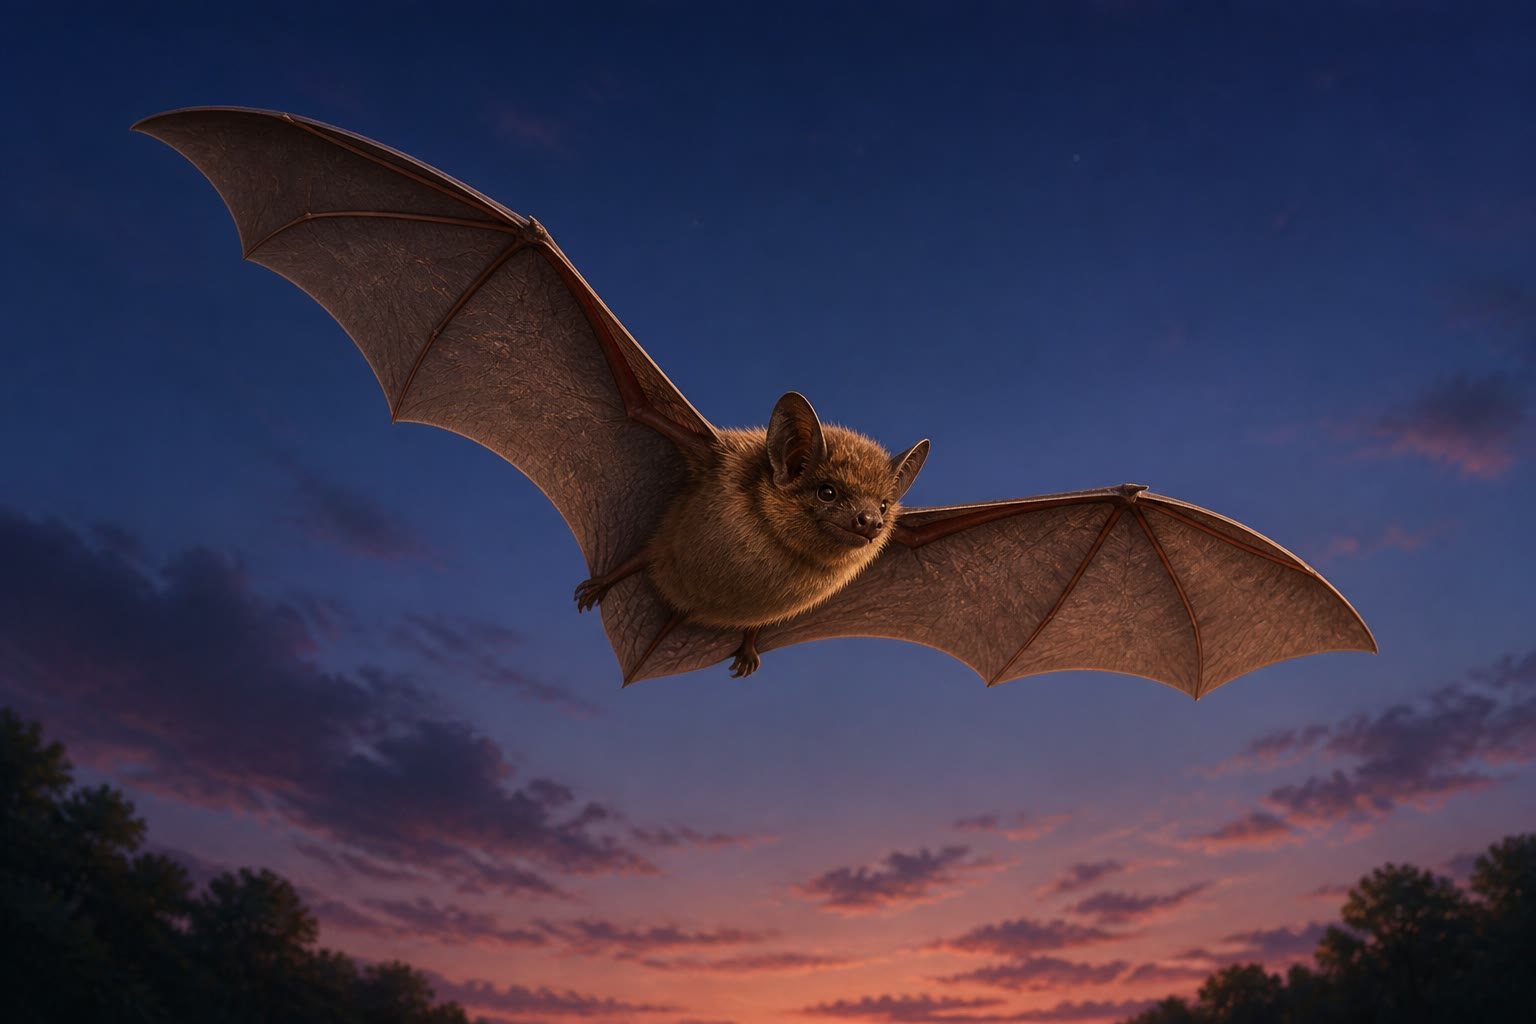
\includegraphics[width=0.6\linewidth]{images/book1/ai/g3-sort-bat.jpg}

{\small Vuela como un ave --- y lleva \omterm{def:g1:animals-around-us:covering}{pelo} sobre unas alas desnudas:
el murciélago, la prueba clásica de clasificar por rasgos y no por
impresiones.}
\end{omfigure}

\begin{method}[Clasificar un animal desconocido]\label{met:g3:sorting-living-things:sort}
\begin{enumerate}
  \item observa el cuerpo: ¿\omterm{def:g1:the-five-senses:sense}{piel}, \omterm{def:g1:animals-around-us:covering}{pelo}, \omterm{def:g1:animals-around-us:covering}{plumas} o escamas? ¿cuántas
        patas? ¿alas? ¿pico?
  \item pregunta por las crías si puedes: ¿\omterm{def:g2:animals-grow-up:born}{leche}? ¿\omterm{def:g2:animals-grow-up:born}{huevos}? ¿una etapa
        de renacuajo?
  \item compara con los grupos de la
        \cref{prop:g3:sorting-living-things:groups} y coloca al \omterm{def:g1:animals-around-us:animal}{animal}
        donde encajen sus \emph{rasgos};
  \item si una impresión (``¡vuela!'') no concuerda con un rasgo
        (``tiene \omterm{def:g1:animals-around-us:covering}{pelo}''), fíate del rasgo.
\end{enumerate}
\end{method}

\section{Las plantas también se clasifican}

\begin{proposition}[Clasificar plantas]\label{prop:g3:sorting-living-things:plants}
Las \omterm{def:g1:plants-around-us:plant}{plantas} se clasifican por sus rasgos igual que los \omterm{def:g1:animals-around-us:animal}{animales}.
\omterm{def:g3:sorting-living-things:criterion}{Criterios} útiles: ¿hace \emph{\omterm{def:g1:plants-around-us:parts}{flores}} y \omterm{def:g2:from-seed-to-plant:seed}{semillas} (la margarita, el
castaño) o no hace ninguna nunca (el helecho, el musgo)? ¿Es su \omterm{def:g1:plants-around-us:parts}{tallo}
blando y verde o leñoso como el tronco de un \emph{árbol}? ¿Son las
\omterm{def:g1:plants-around-us:parts}{hojas} anchas o son agujas como las del pino?
\end{proposition}
\admitted

\begin{example}[Tres rincones del parque]\label{ex:g3:sorting-living-things:park}
En un mismo parque: el rosal --- \omterm{def:g1:plants-around-us:parts}{flores}, \omterm{def:g1:plants-around-us:parts}{tallos} leñosos; el musgo del
muro norte --- ninguna \omterm{def:g1:plants-around-us:parts}{flor} nunca, ningún \omterm{def:g1:plants-around-us:parts}{tallo} de verdad; el pino ---
un árbol con agujas y piñas. Tres \omterm{def:g1:plants-around-us:plant}{plantas}, tres respuestas distintas a
los mismos \omterm{def:g3:sorting-living-things:criterion}{criterios}.
\end{example}

\begin{remark}[Clasificar es el primer paso de una ciencia]\label{rem:g3:sorting-living-things:science}
Los grupos bien clasificados permiten hacer preguntas mejores: todo lo
que es cierto de los \omterm{prop:g3:sorting-living-things:groups}{insectos} en general --- seis patas, cuerpo en
tres partes, a menudo alas --- se sabe de golpe para cientos de miles
de especies a la vez. Capítulos posteriores convertirán la
\omterm{def:g3:sorting-living-things:criterion}{clasificación} en un árbol de familia de todos los \omterm{def:g1:living-or-not:living}{seres vivos} ---
por ahora, aprende a clasificar por lo que se ve.
\end{remark}

\section{Ejercicios}

\begin{exercise}[$\star$]\label{exo:g3:sorting-living-things:1}
¿Qué es un \omterm{def:g3:sorting-living-things:criterion}{criterio}? Da un buen \omterm{def:g3:sorting-living-things:criterion}{criterio} para clasificar \omterm{def:g1:animals-around-us:animal}{animales} y
otro que los biólogos eviten.
\end{exercise}

\begin{exercise}[$\star$]\label{exo:g3:sorting-living-things:2}
Da el rasgo (o los rasgos) que definen cada grupo: \omterm{prop:g3:sorting-living-things:groups}{insectos}, \omterm{prop:g3:sorting-living-things:groups}{peces},
\omterm{prop:g3:sorting-living-things:groups}{aves}, \omterm{prop:g3:sorting-living-things:groups}{mamíferos}.
\end{exercise}

\begin{exercise}[$\star$]\label{exo:g3:sorting-living-things:3}
Coloca cada \omterm{def:g1:animals-around-us:animal}{animal} en su grupo: la abeja, el \omterm{prop:g3:sorting-living-things:groups}{pez} de colores, el
avestruz, la vaca, la rana.
\end{exercise}

\begin{exercise}[$\star$]\label{exo:g3:sorting-living-things:4}
El murciélago vuela. ¿Por qué es un mamífero y no un ave? ¿Qué rasgos
lo deciden?
\end{exercise}

\begin{exercise}[$\star$]\label{exo:g3:sorting-living-things:5}
La ballena vive en el mar. ¿Por qué no es un \omterm{prop:g3:sorting-living-things:groups}{pez}? ¿Qué rasgos lo
deciden?
\end{exercise}

\begin{exercise}[$\star$]\label{exo:g3:sorting-living-things:6}
Una araña tiene ocho patas. ¿Puede ser un insecto? ¿Qué responde el
\omterm{def:g3:sorting-living-things:criterion}{criterio}?
\end{exercise}

\begin{exercise}[$\star$]\label{exo:g3:sorting-living-things:7}
Clasifica estas \omterm{def:g1:plants-around-us:plant}{plantas} con los \omterm{def:g3:sorting-living-things:criterion}{criterios} de la
\cref{prop:g3:sorting-living-things:plants}: la margarita, el musgo,
el pino, el rosal.
\end{exercise}

\begin{exercise}[$\star$]\label{exo:g3:sorting-living-things:8}
Pruébalo: clasifica los \omterm{def:g1:animals-around-us:animal}{animales} de tu calle o de tu jardín --- todos
los que veas en un paseo --- en los grupos de este capítulo. ¿Qué
grupo gana por número?
\end{exercise}

\begin{exercise}[$\star\star$]\label{exo:g3:sorting-living-things:9}
Lea clasifica los \omterm{def:g1:animals-around-us:animal}{animales} en ``mascotas'' y ``\omterm{def:g1:animals-around-us:animal}{animales} salvajes''.
Su amiga clasifica esos mismos \omterm{def:g1:animals-around-us:animal}{animales} en ``\omterm{prop:g3:sorting-living-things:groups}{mamíferos}'' y ``\omterm{prop:g3:sorting-living-things:groups}{aves}''.
¿Qué \omterm{def:g3:sorting-living-things:criterion}{clasificación} es la de un biólogo y por qué? Usa la
\cref{rem:g3:sorting-living-things:why}.
\end{exercise}

\begin{exercise}[$\star\star$]\label{exo:g3:sorting-living-things:10}
Un pingüino nada de maravilla, no puede volar y está cubierto de algo
que parecen tejas brillantes. Una naturalista mira de cerca: las
``tejas'' son \omterm{def:g1:animals-around-us:covering}{plumas} muy apretadas, y hay un pico. Pásale al pingüino
el \cref{met:g3:sorting-living-things:sort}, paso a paso.
\end{exercise}
